% 图 16.1 —— 由 `checks/emit_hand.py` 自动拼出（probe 精测 + prims2 图元分解）
%%
% ⚠ 这是**稿子不是成品**：跑 `checks/checkhand.py 16.1` 看指标 + 看叠合图。
%%
%% ⚠ 待核：
%   · 本图 probe 报出阴影族 2 个 —— **本脚本不生成阴影**（要照原书手写）；prims2 的 strokes 里可能含阴影线，核对时留意别画重
%   · 可疑字形 1 项（空心圈 ⊙ 常被认成字母 o）—— 见文件末
%%
\documentclass[12pt]{standalone}
\usepackage{fontspec}
\setsansfont{Arial}
\newfontfamily\mfallback{DejaVu Sans}
\usepackage{tikz}
\begin{document}
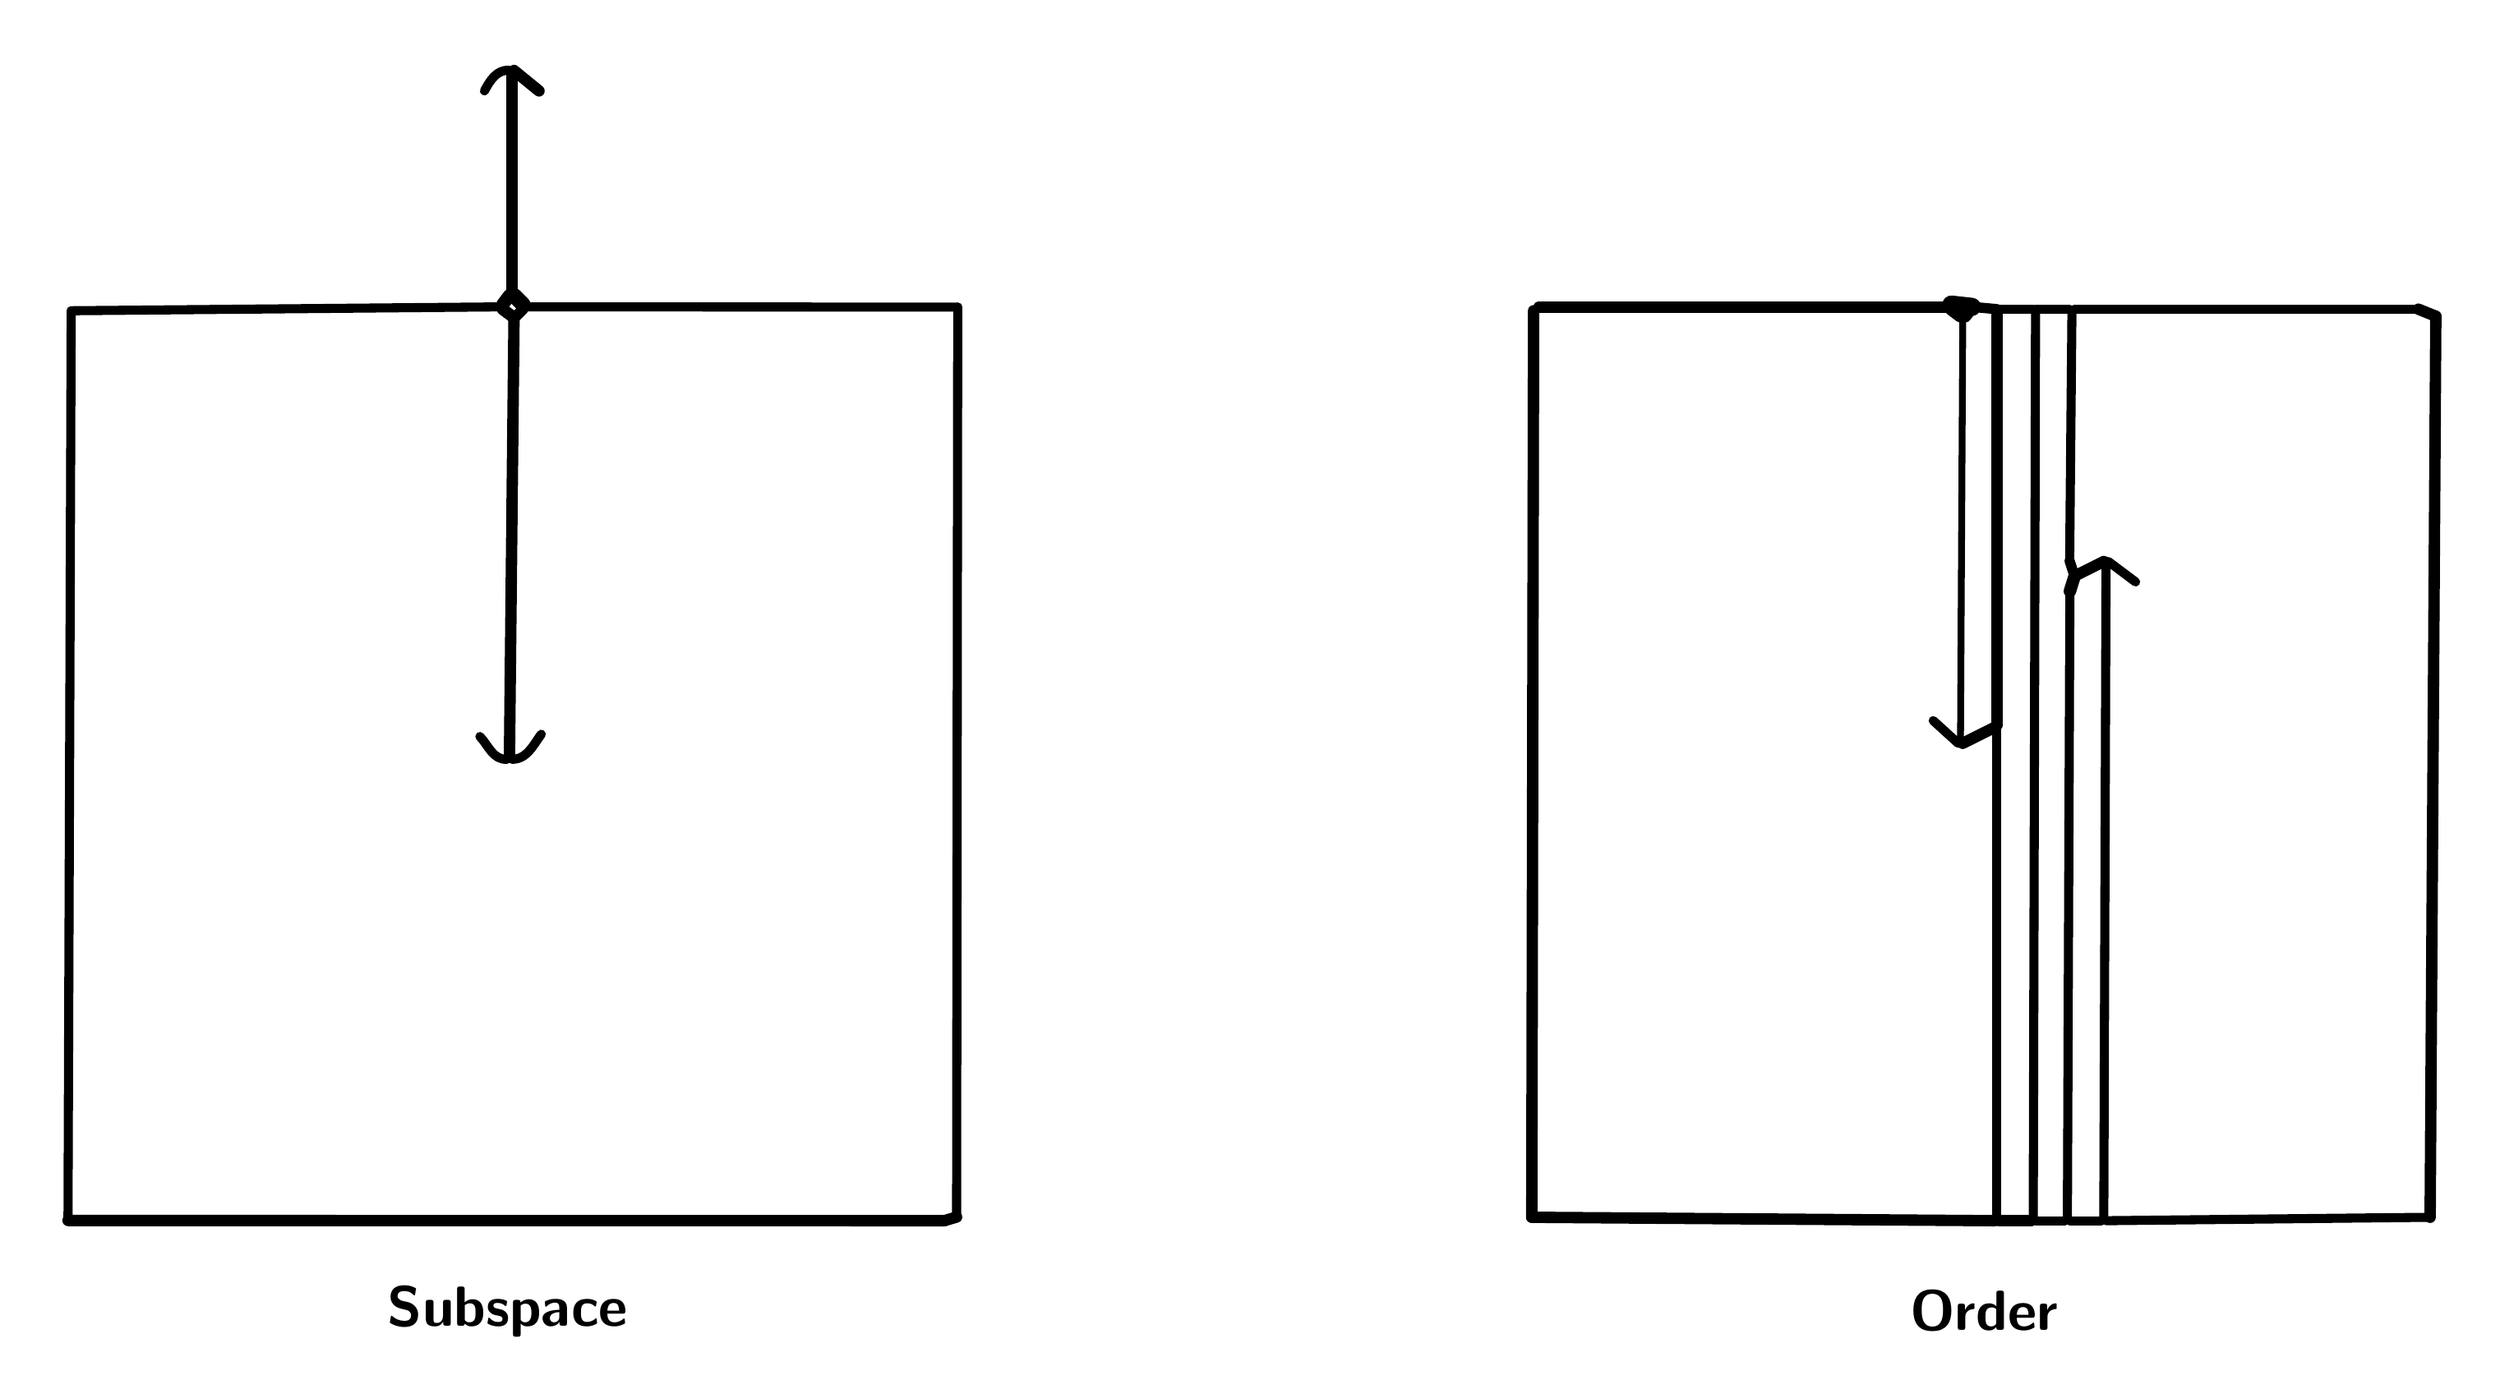
\begin{tikzpicture}[x=1pt, y=-1pt, line width=5.0pt, line cap=round, line join=round]

  %% ════ 直线段（prims2 的 strokes）════
  \draw[line width=5.0pt] (216.0,130.0) -- (214.0,323.0);
  \draw[line width=8.0pt] (857.0,125.0) -- (848.0,124.0);
  \draw[line width=4.5pt] (857.0,125.0) -- (868.0,126.0);
  \draw[line width=5.7pt] (857.0,125.0) -- (854.0,129.0);
  \draw[line width=4.0pt] (900.0,527.0) -- (914.0,527.0);
  \draw[line width=5.0pt] (215.0,119.0) -- (215.0,22.0);
  \draw[line width=5.5pt] (902.0,244.0) -- (900.1,250.1);
  \draw[line width=4.0pt] (900.1,250.1) -- (899.0,526.0);
  \draw[line width=5.0pt] (853.0,317.0) -- (867.0,310.0);
  \draw[line width=4.0pt] (210.0,125.0) -- (21.3,126.7);
  \draw[line width=4.0pt] (21.3,126.7) -- (19.9,526.9);
  \draw[line width=5.0pt] (19.9,526.9) -- (405.2,527.0);
  \draw[line width=5.0pt] (405.2,527.0) -- (410.6,525.4);
  \draw[line width=4.0pt] (410.6,525.4) -- (411.1,125.1);
  \draw[line width=4.0pt] (411.1,125.1) -- (221.0,125.0);
  \draw[line width=4.7pt] (220.0,126.0) -- (217.0,129.0);
  \draw[line width=4.0pt] (885.0,126.0) -- (900.0,126.0);
  \draw[line width=5.0pt] (903.0,243.0) -- (915.0,237.0);
  \draw[line width=5.7pt] (848.0,126.0) -- (852.0,129.0);
  \draw[line width=6.7pt] (216.0,120.0) -- (220.0,124.0);
  \draw[line width=4.0pt] (869.0,126.0) -- (884.0,126.0);
  \draw[line width=4.0pt] (915.0,526.0) -- (916.0,238.0);
  \draw[line width=3.0pt] (853.0,130.0) -- (852.0,316.0);
  \draw[line width=5.7pt] (211.0,124.0) -- (214.0,120.0);
  \draw[line width=5.0pt] (847.0,125.0) -- (666.7,125.0);
  \draw[line width=2.9pt] (666.7,125.0) -- (664.3,126.7);
  \draw[line width=5.0pt] (664.3,126.7) -- (663.5,525.5);
  \draw[line width=5.0pt] (663.5,525.5) -- (867.0,527.0);
  \draw[line width=4.0pt] (917.0,237.0) -- (929.0,246.0);
  \draw[line width=4.5pt] (902.0,243.0) -- (900.0,236.8);
  \draw[line width=4.0pt] (900.0,236.8) -- (901.0,127.0);
  \draw[line width=5.0pt] (883.0,527.0) -- (869.0,527.0);
  \draw[line width=4.0pt] (868.0,311.0) -- (868.0,526.0);
  \draw[line width=4.0pt] (885.0,127.0) -- (884.0,526.0);
  \draw[line width=4.0pt] (885.0,527.0) -- (898.0,527.0);
  \draw[line width=5.0pt] (216.0,21.0) -- (227.0,30.0);
  \draw[line width=4.0pt] (902.0,126.0) -- (1053.3,126.0);
  \draw[line width=5.0pt] (1053.3,126.0) -- (1061.0,129.1);
  \draw[line width=5.0pt] (1061.0,129.1) -- (1058.5,525.5);
  \draw[line width=4.0pt] (1058.5,525.5) -- (916.0,527.0);
  \draw[line width=4.0pt] (840.0,307.0) -- (851.0,317.0);
  \draw[line width=5.2pt] (211.0,126.0) -- (215.0,129.0);
  \draw[line width=5.0pt] (868.0,127.0) -- (868.0,309.0);

  %% ════ 曲线（prims2 的 curves —— 三段式，坐标同为 (y,x)）════
  \draw[line width=4.0pt] (203.0,30.0) .. controls (205.2,25.8) and (208.5,20.3) .. (214.0,21.0);
  \draw[line width=4.0pt] (213.0,324.0) .. controls (206.7,324.4) and (204.8,317.9) .. (201.0,314.0);
  \draw[line width=4.0pt] (215.0,324.0) .. controls (221.7,324.2) and (224.6,317.5) .. (228.0,313.0);

  %% ════ 标签（probe 直接给的 \node 行）════
  %% ⚠ 全部补了 fill=white：文字在最上层，否则与曲线交叉干扰
     \node[anchor=center,inner sep=0pt,fill=white,font=\fontsize{30.5}{38.1}\selectfont] at (213.3,567.0) {\textsf{\textbf{\textit{Subspace}}}};   % box(145,552,136,29)
     \node[anchor=center,inner sep=0pt,fill=white,font=\fontsize{30.3}{37.9}\selectfont] at (862.5,566.5) {\textsf{\textbf{\textit{Order}}}};   % box(824,554,78,24)

  % 钉死画布：否则超出的图元/控制点会把页面撑大，1:1 回比就失准
  \pgfresetboundingbox
  \path[use as bounding box] (0,0) rectangle (1079,591);
\end{tikzpicture}
\end{document}

% ⚠ 待核清单（probe 拿不准，人眼过一遍）：
%   · 未识别/跳过：⑤ 跳过/未识别的字形
